\documentclass[utf8]{beamer}

\usepackage{ufcd} 
% Alternative für englischsprachige Dokumente
%\usepackage[mainlanguage=english]{ufcd}

% Inoffizielle LaTeX-Vorlage für Vorträge
% an der Fakultät für Chemie und Pharmazie
% der Albert-Ludwigs-Universität Freiburg
%
% Diese Vorlage ist lediglich ein Vorschlag, der versucht, sowohl
% typografischen Ansprüchen ansatzweise gerecht zu werden als auch
% nutzbar zu sein.
%
% Jegliche Nutzung auf eigene Verantwortung.
%
% Copyright (c) 2018, Till Biskup

% Schriftart fuer Formeln anpassen: Serifenschrift
\usefonttheme[onlymath]{serif}

% Vektoren: fett, kursiv
\usepackage{bm}
\renewcommand*{\vec}[1]{\bm{#1}}

% Tensoren: serifenlos, fett, kursiv
\DeclareMathAlphabet{\mathbfsf}{\encodingdefault}{\sfdefault}{bx}{sl}
\newcommand*{\tens}[1]{\mathbfsf{#1}}

% Differentialoperator: aufrecht
\newcommand*{\diff}{\mathrm{d}}

% mathematische Konstanten: aufrecht
\newcommand*{\im}{\mathrm{i}}
\newcommand*{\e}{\mathrm{e}}

% für das aufrechte kleine pi: \uppi
\usepackage[Symbolsmallscale]{upgreek}

% Operatoren mit Dach
\newcommand*{\op}[1]{\hat{#1}}

% Dirac-Notation
\newcommand*{\bra}[1]{\left\langle#1\right\rvert}
\newcommand*{\ket}[1]{\left\lvert#1\right\rangle}
\newcommand*{\braket}[2]{\langle#1\lvert#2\rangle}

% Inoffizielle LaTeX-Vorlage für Vorträge
% an der Fakultät für Chemie und Pharmazie
% der Albert-Ludwigs-Universität Freiburg
%
% Diese Vorlage ist lediglich ein Vorschlag, der versucht, sowohl
% typografischen Ansprüchen ansatzweise gerecht zu werden als auch
% nutzbar zu sein.
%
% Jegliche Nutzung auf eigene Verantwortung.
%
% Copyright (c) 2018, Till Biskup

%% Anführungszeichen sprachabhängig und "intelligent"
\usepackage[autostyle]{csquotes}

%% typografisch korrekte Tabellen
\usepackage{booktabs}

%% Korrekter Satz von Zahlen und Einheiten
\usepackage{siunitx}

% Komma als Dezimaltrennzeichen im Text (unabhängig von der Eingabe)
\sisetup{output-decimal-marker={,}}

% Befehl für Quellenangaben
\renewcommand*{\thefootnote}{}
\renewcommand*{\footnoterule}{\rule{0cm}{0cm}}
% Quellenangaben frei formatierbar, rechtsbündig unten auf der Seite
\newcommand*{\quelle}[1]{\footnotetext{\raggedleft{\tiny #1}}}

%% Pakete für zusätzliche Symbole
\usepackage{pifont}

%% Logische Textauszeichnung
% fremdsprachige Begriffe kursiv
\newcommand*{\foreign}[1]{\emph{#1}}

% LaTeX-Paketnamen in Schreibmaschinenschrift (dicktengleich)
\newcommand*{\package}[1]{\texttt{#1}}

% (LaTeX-)Befehle in Schreibmaschinenschrift (dicktengleich)
\newcommand*{\command}[1]{\texttt{#1}}

% Datei- und Verzeichnisnamen in Schreibmaschinenschrift
\newcommand*{\filename}[1]{\texttt{#1}}

% Inoffizielle LaTeX-Vorlage für Vorträge
% an der Fakultät für Chemie und Pharmazie
% der Albert-Ludwigs-Universität Freiburg
%
% Diese Vorlage ist lediglich ein Vorschlag, der versucht, sowohl
% typografischen Ansprüchen ansatzweise gerecht zu werden als auch
% nutzbar zu sein.
%
% Jegliche Nutzung auf eigene Verantwortung.
%
% Copyright (c) 2018, Till Biskup

% Farbe der Marker für Aufzählungslisten
\setbeamertemplate{itemize item}{\color{Uni-Rot}{$\blacktriangleright$}\;}
\setbeamertemplate{itemize subitem}{%
 \raisebox{.25ex}{\scalebox{.7}{\color{Uni-Grau}{$\blacksquare$}}}\;}

% Ausschalten der Navigationselemente
\beamertemplatenavigationsymbolsempty

% Inoffizielle LaTeX-Vorlage für Vorträge
% an der Fakultät für Chemie und Pharmazie
% der Albert-Ludwigs-Universität Freiburg
%
% Diese Vorlage ist lediglich ein Vorschlag, der versucht, sowohl
% typografischen Ansprüchen ansatzweise gerecht zu werden als auch
% nutzbar zu sein.
%
% Jegliche Nutzung auf eigene Verantwortung.
%
% Copyright (c) 2018, Till Biskup

%% Einbinden von Quellcode
\usepackage{listings}

% Unterstützte Sprachen sollten einmal geladen werden
\lstloadlanguages{[LaTeX]TeX,Python,Matlab}

\lstset{
  basicstyle=\footnotesize\ttfamily, % Standardschrift
  showstringspaces=false,            % Leerzeichen in Strings anzeigen?
  tabsize=2,                         % Größe von Tabs
  breaklines=true,                   % Zeilen werden umgebrochen
  prebreak=\dots,                    % drei Punkte vor dem Zeilenumbruch
  keywordstyle=\color{blue},         % Stil der Schlüsselworte
  frame=tb,                          % Rahmenlinie oben und unten
  belowcaptionskip=2ex               % Platz unterhalb der Überschrift
}

% Umlaute dürfen direkt in den Listings eingegeben werden
\lstset{
  literate=%
  {Ö}{{\"O}}1
  {Ä}{{\"A}}1
  {Ü}{{\"U}}1
  {ß}{{\ss}}1
  {ü}{{\"u}}1
  {ä}{{\"a}}1
  {ö}{{\"o}}1
  {~}{{\textasciitilde}}1,
  extendedchars=true
}

\lstdefinestyle{latex}{
  language=[LaTeX]TeX,
  commentstyle=\color{gray},       % Stil der Kommentare
  numbers=left,                    % Ort der Zeilennummern
  numberstyle=\tiny,               % Stil der Zeilennummern
  stepnumber=2,                    % Abstand zwischen den Zeilennummern
  numbersep=5pt,                   % Abstand der Nummern zum Text
  xleftmargin=17pt,
  framexleftmargin=17pt
}

% Stil für den Anhang mit kleinerer Schriftgröße
\lstdefinestyle{latex-appendix}{
  language=[LaTeX]TeX,
  basicstyle=\scriptsize\ttfamily, % Standardschrift
  commentstyle=\color{gray},       % Stil der Kommentare
  numbers=left,                    % Ort der Zeilennummern
  numberstyle=\tiny,               % Stil der Zeilennummern
  stepnumber=2,                    % Abstand zwischen den Zeilennummern
  numbersep=5pt,                   % Abstand der Nummern zum Text
  xleftmargin=17pt,
  framexleftmargin=17pt,
  morekeywords={lstset,KOMAoptions,addkomafont,setcapindent,%
    graphicspath,setstretch,DeclareGraphicsExtensions,addtokomafont,%
    DeclareMathAlphabet,addbibresource,DeclareFieldFormat,%
    renewbibmacro,lstloadlanguages,lstdefinestyle,hypersetup,color,%
    lvert,rvert,sisetup,appto}
}


% Inoffizielle LaTeX-Vorlage für Vorträge
% an der Fakultät für Chemie und Pharmazie
% der Albert-Ludwigs-Universität Freiburg
%
% Diese Vorlage ist lediglich ein Vorschlag, der versucht, sowohl
% typografischen Ansprüchen ansatzweise gerecht zu werden als auch
% nutzbar zu sein.
%
% Jegliche Nutzung auf eigene Verantwortung.
%
% Copyright (c) 2018, Till Biskup

%% Grafiken einbinden
\usepackage{graphicx}

% (relative) Pfade zu den Dateien
\graphicspath{{./Abbildungen/eigene/}{./Abbildungen/fremde/}}

% Reihenfolge der Dateiformate
\DeclareGraphicsExtensions{.pdf,.jpg,.png}


%% Titeldaten
\title[Präsentationen mit \LaTeX{}]{Vorlage für Präsentationen mit \LaTeX{}}
\subtitle[]{Ein kurzer Überflug}
\author[H. Wurst]{Hans Wurst}
\date{11.11.2011}
\institute[IPC]{Institut für Physikalische Chemie\\ Albert-Ludwigs-Universität Freiburg}
\subject{Vorlage für Präsentationen}

\begin{document}

\begin{frame}[plain]
% Wenn Navigationssymbole gewünscht sind, auf der Titelseite ausschalten
%\setbeamertemplate{navigation symbols}{}
\titlepage
\end{frame}


\begin{frame}
\frametitle{Überblick}

\tableofcontents

\end{frame}


\section{Motivation}


\begin{frame}
\frametitle{Motivation}
\framesubtitle{Warum nur habe ich mir das ans Bein gebunden?}

\begin{itemize}
\item Titel sollten aussagekräftig und kurz (einzeilig) sein.
\begin{itemize}
\item Untertitel sind rein optional.
\end{itemize}

\item möglichst keinen Fließtext, sondern nur Stichpunkte
\begin{itemize}
\item nicht mehr als zwei Ebenen von Stichpunkten
\end{itemize}
\end{itemize}

\begin{itemize}
\setbeamertemplate{itemize item}{\color{Mittel-Gruen}{\ding{56}\;}}
\item Symbole lassen sich für Listen umdefinieren.
\item Das kann mitunter hilfreich sein.
\setbeamertemplate{itemize item}{\color{Uni-Rot}{\ding{52}\,}}
\item Umdefinieren geht auch innerhalb einer Liste.
\end{itemize}

\begin{itemize}
\setbeamertemplate{itemize item}{\color{Uni-Rot}{\ding{52}\,}}
\item Oft sind aber zwei unabhängige Listen besser.
\item Zumal dann automatisch ein kleiner Abstand entsteht.
\end{itemize}

\end{frame}


\section{Theorie}


\begin{frame}[t]
\frametitle{Theorie}
\framesubtitle{Darf's ein bisschen Goethe sein?}

\begin{quote}
Grau, teurer Freund, ist alle Theorie,\\
Und grün des Lebens goldner Baum.
\quelle{J.W. von Goethe: Faust 1, Studierzimmer. (Mephistopheles)}
\end{quote}

\begin{align*}
\hat{H}\Psi = E\Psi
\end{align*}

\begin{itemize}
\item \package{amsmath} wird von \package{beamer} bereits geladen.
\item mathematische Formeln in \textrm{Serifenschrift} setzen
\begin{itemize}
\item Standardschrift auf Folien sonst serifenlos
\end{itemize}
\end{itemize}

\end{frame}


\section{Ergebnisse}


\begin{frame}[t]
\frametitle{Ergebnisse}
\framesubtitle{Ich wünscht', ich hätte was geschafft \ldots}

\begin{columns}[T]
\begin{column}{.45\textwidth}
\structure{erste Spalte}

\begin{itemize}
\item gut geeignet zur Anordnung von\\ Text und Bild
\item relative Ausrichtung\\ optional möglich
\item Folie ist insgesamt oben bündig ausgerichtet
\end{itemize}

\end{column}
%
\begin{column}{.45\textwidth}
\structure{zweite Spalte}

\vspace*{1ex}

\emph{hier könnte ein Bild stehen}

\begin{itemize}
\item Bilder einfügen wie üblich über \command{includegraphics}
\item meist keine \command{figure}-Umgebung drum herum
\end{itemize}

\end{column}
\end{columns}

\end{frame}


\begin{frame}[t]
\frametitle{Ergebnisse}
\framesubtitle{Weil ich nichts zu sagen habe, zeige ich ein (fremdes) Bild}

\begin{columns}[T]
\begin{column}{.5\textwidth}

\structure{Titel:}

\enquote{fMRI testing showed that subjects who don't agree to participate are much more likely to escape from the machine mid-scan.}

\end{column}
%
\begin{column}{.4\textwidth}


\includegraphics[width=\textwidth]{xkcd-1999-selection_effect}

\end{column}
\end{columns}
\quelle{\textcopyright{} Randall Munroe, CC-By-NC, \url{https://www.xkcd.com/1999/}}

\end{frame}


\begin{frame}
\frametitle{Ergebnisse}
\framesubtitle{Beispiele für die unterschiedlichen vordefinierten Blockumgebungen}

\begin{block}{Blockname}
Das ist eine \command{block}-Umgebung.
\end{block}

\begin{alertblock}{Blockname}
Das ist eine \command{alertblock}-Umgebung.
\end{alertblock}

\begin{exampleblock}{Blockname}
Das ist eine \command{exampleblock}-Umgebung.
\end{exampleblock}

\end{frame}


\begin{frame}
\frametitle{Ergebnisse}
\framesubtitle{Beispiel für ein formatfüllendes Bild}

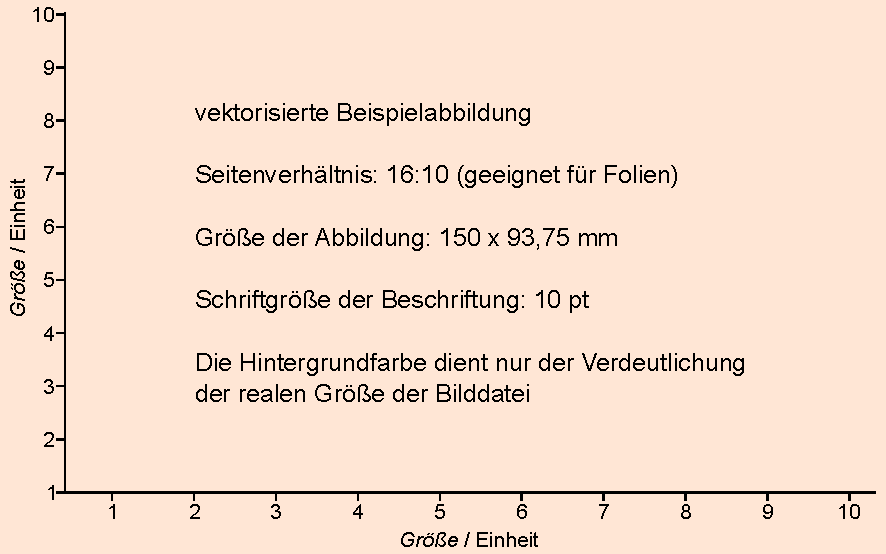
\includegraphics[width=\textwidth]{Beispielabbildung}

\end{frame}


\begin{frame}[fragile]
\frametitle{Ergebnisse}
\framesubtitle{Quellcode-Listings bedürfen besonderer Behandlung}

\begin{lstlisting}[language=Python]
def hello():
    """Print "Hello World" and return None"""
    print("Hello World")

# main program
hello()
\end{lstlisting}

\begin{itemize}
\item Quellcode-Listings (und alle \command{verbatim}-Umgebungen)\\ nur über Option \command{fragile} für \command{frame} möglich
\item Anderenfalls gibt \LaTeX{} einen Fehler aus.
\end{itemize}

\end{frame}


\section{Zusammenfassung}


\begin{frame}
\frametitle{Zusammenfassung}
\framesubtitle{Wie sie sehen, sehen sie nichts.}

\structure{Listen lassen sich schrittweise aufdecken:}

\begin{itemize}[<+->]
\item Am Anfang hatte mein Betreuer\\ eine vielversprechende Idee.
\begin{itemize}
\item ...und deshalb habe ich mich auch darauf eingelassen.
\end{itemize}

\item Dann hat er mich ein Semester lang versklavt.

\item Rausgekommen ist auch nichts.

\item Aber mit diesem Vortrag habe ich meine Pflicht getan.
\end{itemize}

\begin{itemize}
\item<6-> Das geht auch manuell.
\begin{itemize}
\item Vorteil: Unterpunkte werden gleichzeitig aufgedeckt.
\item Nachteil: Reihenfolge muss \alert<7->{explizit angegeben} werden
\end{itemize}
\end{itemize}

\end{frame}


\begin{frame}
\frametitle{Danksagung}

Meerschweinchen\\
Goldfisch\\
Eltern\\
\ldots

\vspace*{\fill}

\begin{center}
\structure{That does it -- screw you, guys I'm goin' home!}
\end{center}

\end{frame}

\newcounter{finalframe}
\setcounter{finalframe}{\value{framenumber}}
\appendix


\begin{frame}
\frametitle{Anhang}
\framesubtitle{Was ich noch gesagt hätte, wenn noch Zeit gewesen wäre}

Things you never wanted to know -- but were forced to find out.

\end{frame}

\setcounter{framenumber}{\value{finalframe}}
\end{document}